\documentclass[tikz,border=0pt]{standalone}
\usepackage[american]{circuitikz}
\usetikzlibrary{arrows.meta,calc,positioning,decorations.pathmorphing,patterns}
\definecolor{zyloTeal}{HTML}{174A5B}
\definecolor{zyloTealTwo}{HTML}{246B7A}
\definecolor{zyloInk}{HTML}{1F2933}
\definecolor{zyloSoft}{HTML}{EAF4F4}
\definecolor{zyloPaper}{HTML}{F8FAFB}
\definecolor{zyloLine}{HTML}{44606B}
\definecolor{zyloOrange}{HTML}{D97706}
\begin{document}
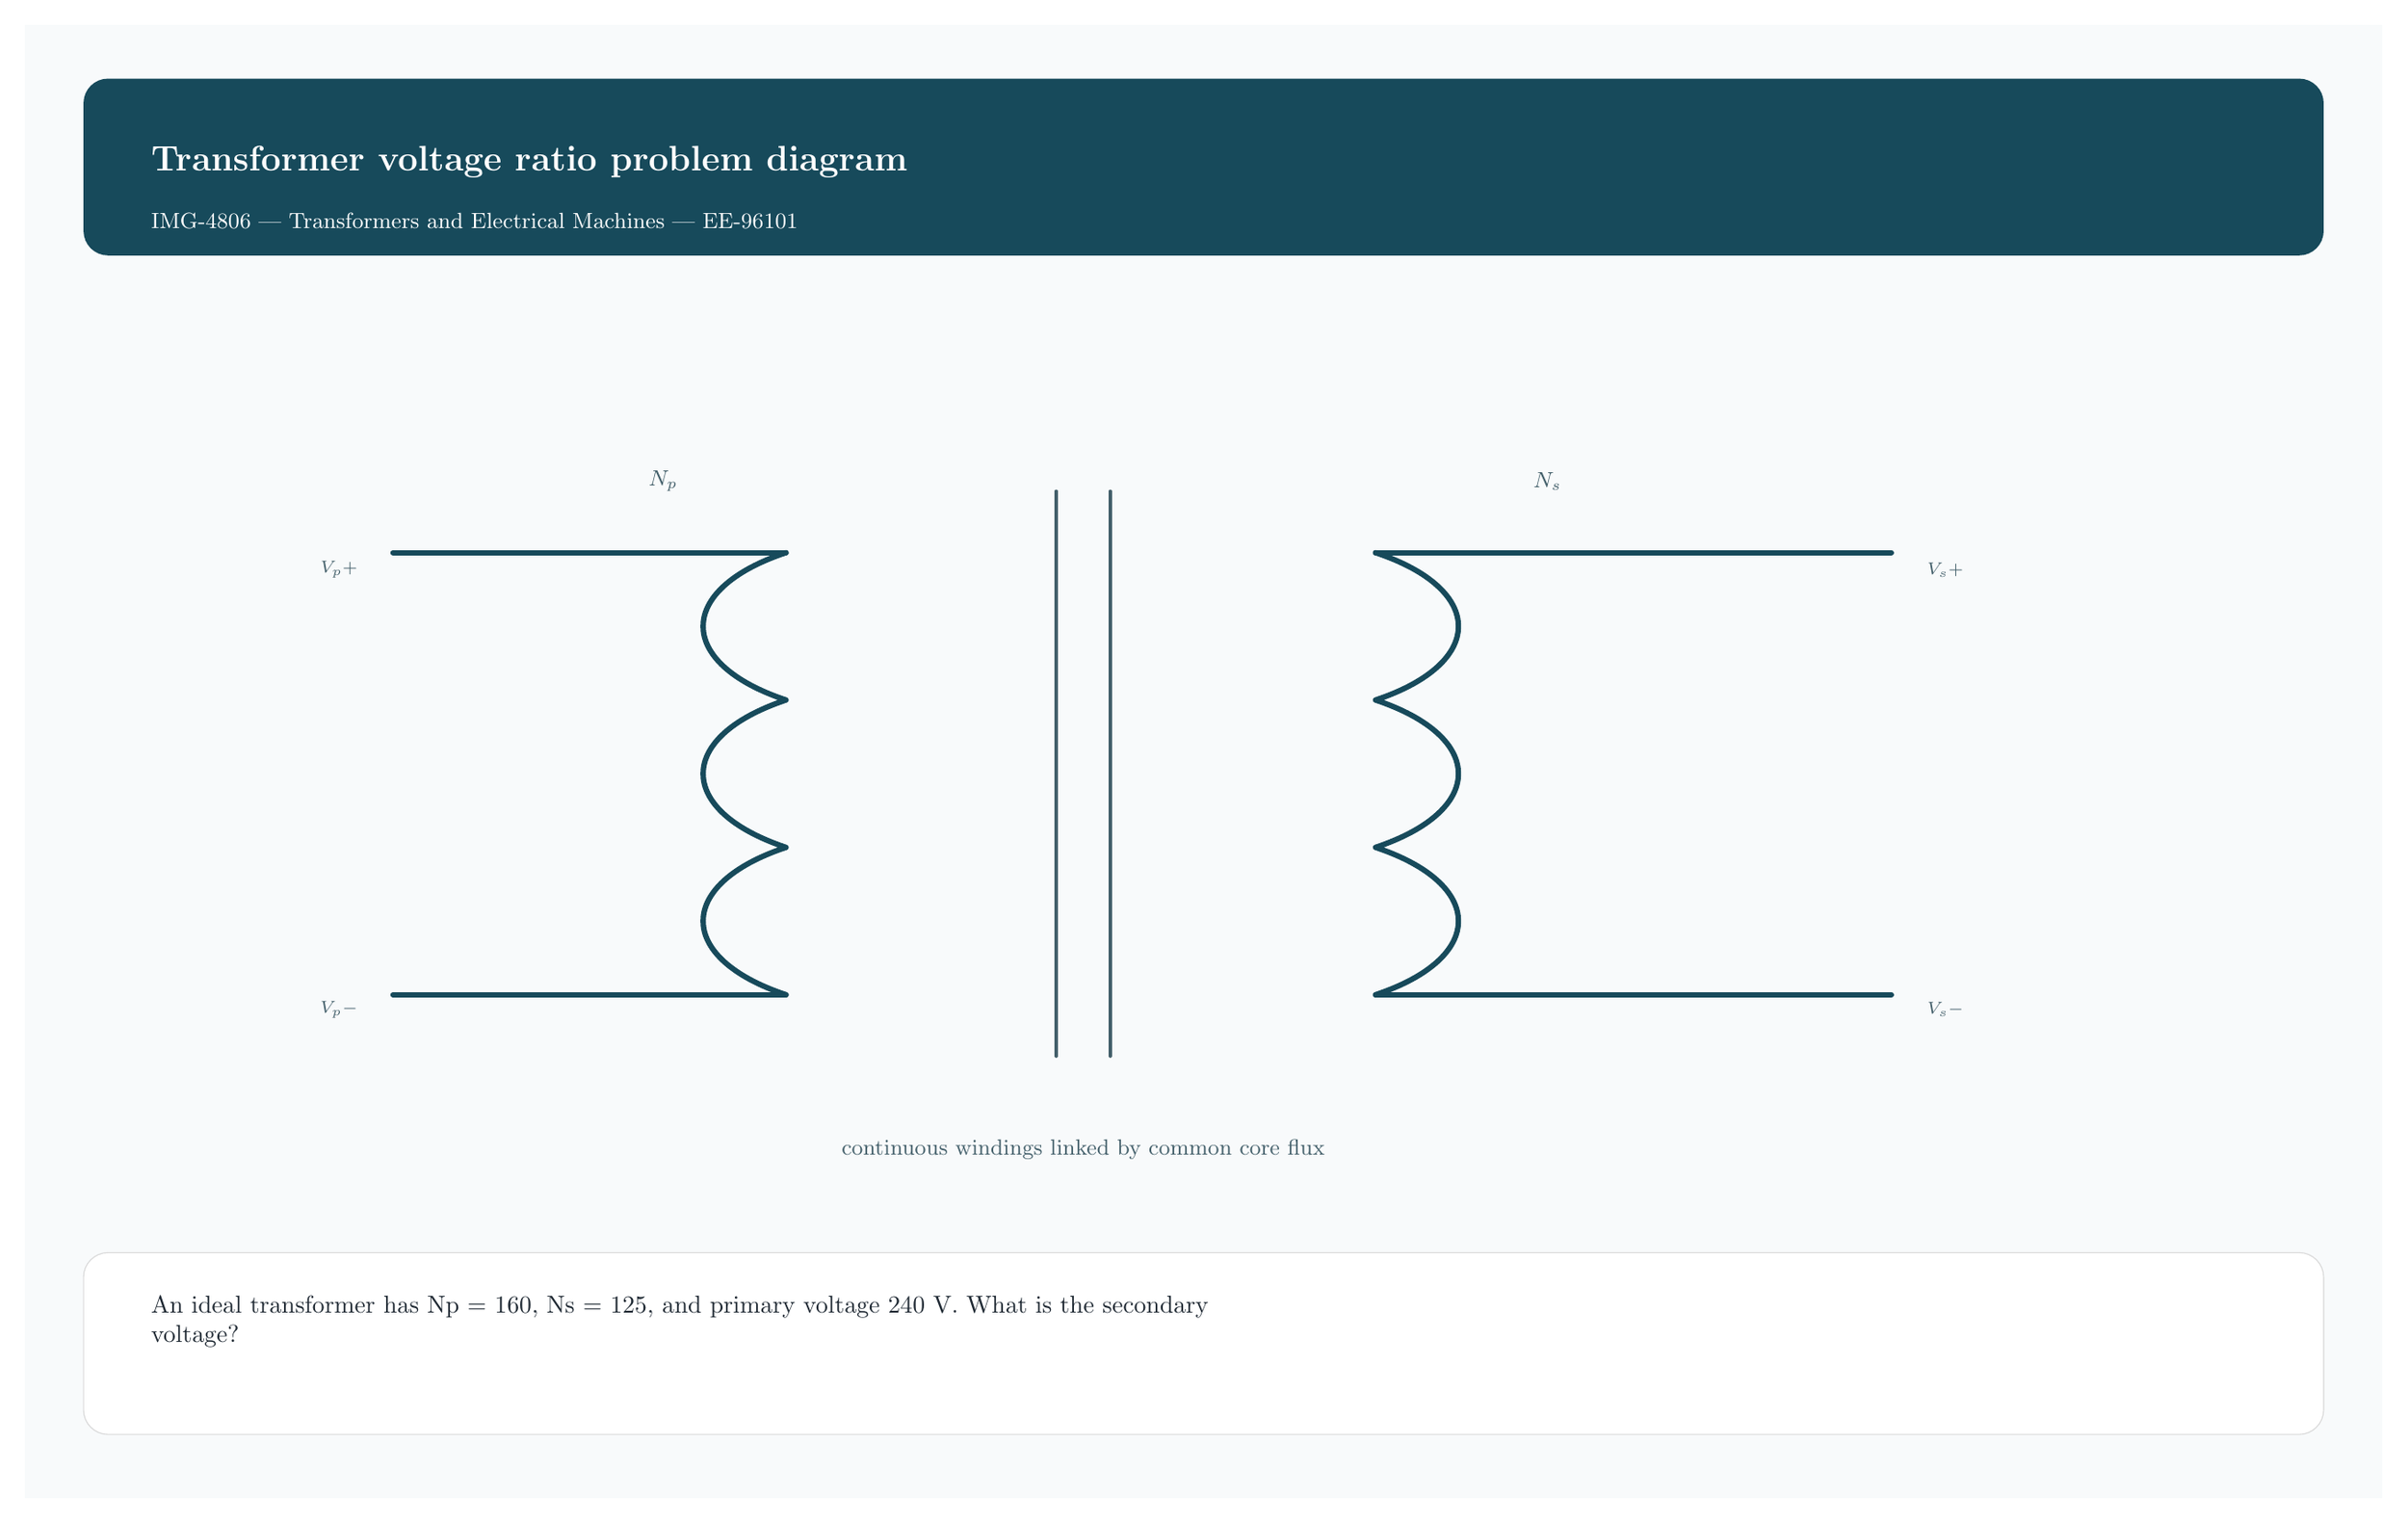
\begin{tikzpicture}[x=1pt,y=-1pt,>=Latex,line cap=round,line join=round]
\path[fill=zyloPaper] (0,0) rectangle (960,600);
\path[fill=zyloTeal,rounded corners=10pt] (24,22) rectangle (936,94);
\node[anchor=west,text=white,font=\bfseries\Large] at (48,56) {Transformer voltage ratio problem diagram};
\node[anchor=west,text=white!82,font=\small] at (48,80) {IMG-4806 | Transformers and Electrical Machines | EE-96101};
\tikzset{wire/.style={draw=zyloTeal,line width=2.2pt},thinwire/.style={draw=zyloLine,line width=1.35pt},accent/.style={draw=zyloOrange,line width=2.2pt},box/.style={draw=zyloTealTwo,fill=zyloSoft,line width=1.5pt,rounded corners=8pt}}
\draw[wire] (150,215) -- (310,215);
\draw[wire] (310,215) .. controls (265,230) and (265,260) .. (310,275) .. controls (265,290) and (265,320) .. (310,335) .. controls (265,350) and (265,380) .. (310,395);
\draw[wire] (310,395) -- (150,395);
\draw[thinwire] (420,190) -- (420,420); \draw[thinwire] (442,190) -- (442,420);
\draw[wire] (550,215) -- (760,215);
\draw[wire] (550,215) .. controls (595,230) and (595,260) .. (550,275) .. controls (595,290) and (595,320) .. (550,335) .. controls (595,350) and (595,380) .. (550,395);
\draw[wire] (550,395) -- (760,395);
\node[font=\small,text=zyloLine] at (260,186) {$N_p$}; \node[font=\small,text=zyloLine] at (620,186) {$N_s$};
\node[font=\scriptsize,text=zyloLine] at (128,222) {$V_p+$}; \node[font=\scriptsize,text=zyloLine] at (128,401) {$V_p-$};
\node[font=\scriptsize,text=zyloLine] at (782,222) {$V_s+$}; \node[font=\scriptsize,text=zyloLine] at (782,401) {$V_s-$};
\node[font=\small,text=zyloLine] at (431,458) {continuous windings linked by common core flux};
\path[draw=black!15,fill=white,rounded corners=10pt] (24,500) rectangle (936,574);
\node[anchor=west,text width=860pt,align=left,text=zyloInk,font=\normalsize] at (48,528) {An ideal transformer has Np = 160, Ns = 125, and primary voltage 240 V. What is the secondary\\voltage?};
\end{tikzpicture}
\end{document}
